% make sure you have the VPN on, so that latex can load packages on the fly
% upload the project folder to overleaf

\documentclass[12pt,twoside]{scrreport}

\usepackage[a4paper,inner=1.5in,outer=1in,top=1in,bottom=1in]{geometry}

\usepackage{ipsum}
\usepackage{subcaption}


\usepackage{chngcntr} % Allows customization of counters
\counterwithout{figure}{chapter} % Make figure numbers independent of chapters
\counterwithout{table}{chapter}  % Make table numbers independent of chapters

\usepackage[printonlyused]{acronym}

% graphics package
\usepackage{graphicx} 

\usepackage[ngerman, english]{babel}

% enhanced citation package 
\usepackage{natbib}
\bibpunct{(}{)}{;}{a}{}{,}  % to adjust punctuation in references


% adjust caption properties
\usepackage{caption} 
\captionsetup[table]{position=top,justification=justified,singlelinecheck=false,format=plain}
\captionsetup[figure]{position=below,justification=justified,singlelinecheck=false,format=plain}

\captionsetup{
	labelfont=bf,         % Bold label (e.g., Table 2:)
	textfont=normalfont,  % Normal font for the text
	labelsep=colon,       % Colon after "Table X" or "Figure X"
	indention=0pt         % No indentation on the second and following lines
}



% hyperrefs on, with nicer colors
\usepackage{color}
\usepackage{xcolor}
\usepackage[]{hyperref}
\definecolor{darkblue}{rgb}{0,0,.5}
\hypersetup{colorlinks=true, breaklinks=true, linkcolor=darkblue, menucolor=darkblue, urlcolor=darkblue, citecolor=darkblue}

% enhanced tables
\usepackage{multicol}              
\usepackage{multirow}
\usepackage{booktabs} 

% For displaying code
\usepackage{listings}

\usepackage{tikz}

% Define custom settings for R code
%\lstset{
	%language=R,
	%basicstyle=\ttfamily\footnotesize,
	%showstringspaces=false,
	%breaklines=true,
	%frame=single,
	%numbers=left,
	%numberstyle=\tiny\color{gray},
	%captionpos=b
%}

% Commands for formatting R elements
\newcommand{\pkg}[1]{`#1'}
\newcommand{\fn}[2][]{\textit{#2(}#1\textit{)}}
\newcommand{\val}[1]{\texttt{#1}}


\usepackage{float}

%Tilde ~
\usepackage{textcomp}

%\setcounter{secnumdepth}{3}
%\setcounter{tocdepth}{4}
\begin{document}
\pagenumbering{gobble}
\begin{titlepage}
% Symmetrical margins for title page
\newgeometry{top=1in,bottom=1in,left=1in,right=1in} 
\selectlanguage{ngerman}
\begin{center}
% UR Logo
\begin{tikzpicture}[scale=0.5]
	\begin{pgfscope}
		\definecolor{eps2pgf_color}{RGB}{142,142,141}\pgfsetstrokecolor{eps2pgf_color}\pgfsetfillcolor{eps2pgf_color}
		\pgfpathmoveto{\pgfqpoint{2.5cm}{0cm}}
		\pgfpathcurveto{\pgfqpoint{3.881cm}{0cm}}{\pgfqpoint{5cm}{1.119cm}}{\pgfqpoint{5cm}{2.5cm}}
		\pgfpathcurveto{\pgfqpoint{5cm}{3.881cm}}{\pgfqpoint{3.881cm}{5cm}}{\pgfqpoint{2.5cm}{5cm}}
		\pgfpathcurveto{\pgfqpoint{1.119cm}{5cm}}{\pgfqpoint{0cm}{3.881cm}}{\pgfqpoint{0cm}{2.5cm}}
		\pgfpathcurveto{\pgfqpoint{0cm}{1.119cm}}{\pgfqpoint{1.119cm}{0cm}}{\pgfqpoint{2.5cm}{0cm}}
		\pgfusepath{fill}
		\definecolor{eps2pgf_color}{gray}{1}\pgfsetstrokecolor{eps2pgf_color}\pgfsetfillcolor{eps2pgf_color}
		\pgfpathmoveto{\pgfqpoint{3.023cm}{2.542cm}}
		\pgfpathlineto{\pgfqpoint{3.64cm}{2.542cm}}
		\pgfpathlineto{\pgfqpoint{3.64cm}{1.194cm}}
		\pgfpathcurveto{\pgfqpoint{3.64cm}{0.996cm}}{\pgfqpoint{3.67cm}{0.853cm}}{\pgfqpoint{3.728cm}{0.765cm}}
		\pgfpathcurveto{\pgfqpoint{3.787cm}{0.677cm}}{\pgfqpoint{3.881cm}{0.633cm}}{\pgfqpoint{4.01cm}{0.633cm}}
		\pgfpathcurveto{\pgfqpoint{4.143cm}{0.633cm}}{\pgfqpoint{4.243cm}{0.68cm}}{\pgfqpoint{4.31cm}{0.775cm}}
		\pgfpathcurveto{\pgfqpoint{4.377cm}{0.869cm}}{\pgfqpoint{4.411cm}{1.009cm}}{\pgfqpoint{4.411cm}{1.194cm}}
		\pgfpathlineto{\pgfqpoint{4.411cm}{2.542cm}}
		\pgfpathlineto{\pgfqpoint{5cm}{2.542cm}}
		\pgfpathlineto{\pgfqpoint{5cm}{1.194cm}}
		\pgfpathcurveto{\pgfqpoint{5cm}{0.853cm}}{\pgfqpoint{4.918cm}{0.597cm}}{\pgfqpoint{4.753cm}{0.426cm}}
		\pgfpathcurveto{\pgfqpoint{4.588cm}{0.257cm}}{\pgfqpoint{4.341cm}{0.172cm}}{\pgfqpoint{4.011cm}{0.172cm}}
		\pgfpathcurveto{\pgfqpoint{3.684cm}{0.172cm}}{\pgfqpoint{3.437cm}{0.257cm}}{\pgfqpoint{3.271cm}{0.428cm}}
		\pgfpathcurveto{\pgfqpoint{3.106cm}{0.6cm}}{\pgfqpoint{3.023cm}{0.855cm}}{\pgfqpoint{3.023cm}{1.194cm}}
		\pgfpathlineto{\pgfqpoint{3.023cm}{2.542cm}}
		\pgfusepath{fill}
		\definecolor{eps2pgf_color}{RGB}{142,142,141}\pgfsetstrokecolor{eps2pgf_color}\pgfsetfillcolor{eps2pgf_color}
		\pgfpathmoveto{\pgfqpoint{5cm}{2.544cm}}
		\pgfpathlineto{\pgfqpoint{5.921cm}{2.544cm}}
		\pgfpathcurveto{\pgfqpoint{6.228cm}{2.544cm}}{\pgfqpoint{6.455cm}{2.495cm}}{\pgfqpoint{6.603cm}{2.395cm}}
		\pgfpathcurveto{\pgfqpoint{6.752cm}{2.296cm}}{\pgfqpoint{6.826cm}{2.144cm}}{\pgfqpoint{6.826cm}{1.941cm}}
		\pgfpathcurveto{\pgfqpoint{6.826cm}{1.791cm}}{\pgfqpoint{6.787cm}{1.668cm}}{\pgfqpoint{6.708cm}{1.571cm}}
		\pgfpathcurveto{\pgfqpoint{6.63cm}{1.475cm}}{\pgfqpoint{6.517cm}{1.41cm}}{\pgfqpoint{6.37cm}{1.377cm}}
		\pgfpathcurveto{\pgfqpoint{6.491cm}{1.333cm}}{\pgfqpoint{6.589cm}{1.206cm}}{\pgfqpoint{6.663cm}{0.998cm}}
		\pgfpathlineto{\pgfqpoint{6.663cm}{0.996cm}}
		\pgfpathlineto{\pgfqpoint{6.94cm}{0.228cm}}
		\pgfpathlineto{\pgfqpoint{6.296cm}{0.228cm}}
		\pgfpathlineto{\pgfqpoint{6.093cm}{0.863cm}}
		\pgfpathcurveto{\pgfqpoint{6.06cm}{0.964cm}}{\pgfqpoint{6.015cm}{1.035cm}}{\pgfqpoint{5.959cm}{1.075cm}}
		\pgfpathcurveto{\pgfqpoint{5.902cm}{1.113cm}}{\pgfqpoint{5.814cm}{1.133cm}}{\pgfqpoint{5.695cm}{1.133cm}}
		\pgfpathlineto{\pgfqpoint{5.605cm}{1.133cm}}
		\pgfpathlineto{\pgfqpoint{5.605cm}{0.228cm}}
		\pgfpathlineto{\pgfqpoint{5cm}{0.228cm}}
		\pgfpathclose
		\pgfpathmoveto{\pgfqpoint{5.605cm}{2.137cm}}
		\pgfpathlineto{\pgfqpoint{5.605cm}{1.543cm}}
		\pgfpathlineto{\pgfqpoint{5.822cm}{1.543cm}}
		\pgfpathcurveto{\pgfqpoint{5.956cm}{1.543cm}}{\pgfqpoint{6.056cm}{1.567cm}}{\pgfqpoint{6.123cm}{1.616cm}}
		\pgfpathcurveto{\pgfqpoint{6.189cm}{1.664cm}}{\pgfqpoint{6.223cm}{1.737cm}}{\pgfqpoint{6.223cm}{1.834cm}}
		\pgfpathcurveto{\pgfqpoint{6.223cm}{1.938cm}}{\pgfqpoint{6.185cm}{2.015cm}}{\pgfqpoint{6.111cm}{2.064cm}}
		\pgfpathcurveto{\pgfqpoint{6.037cm}{2.113cm}}{\pgfqpoint{5.919cm}{2.137cm}}{\pgfqpoint{5.758cm}{2.137cm}}
		\pgfpathlineto{\pgfqpoint{5.605cm}{2.137cm}}
		\pgfusepath{fill}
	\end{pgfscope}
\end{tikzpicture}

\vfill

{\LARGE \textbf{Extending the \pkg{cito} package: deep convolutional neural networks in ecology}}

\vfill

{\LARGE \textbf{Masterarbeit}}

\vspace{0.5cm}
\large
zur Erlangung des akademischen Grades\\
Master of Science\\
in Computational Science\\
an der Fakultät für Physik\\
der Universität Regensburg
\vfill

\end{center}

\begin{tabular}{ll}
%Eingereicht bei: & Prof.\ Dr.\ Florian Hartig \\
%& Lehrstuhl für Theoretische Ökologie \vspace{5mm}\\

Vorgelegt von: & Armin Schenk \\
& Matrikelnummer: 2037367 \\

Erstgutachter: & Prof. Dr. Florian Hartig\\
Zweitgutachter: & Prof. Dr. Rainer Spang \vspace{5mm}\\

Eingereicht am: & \today\\
\end{tabular}
% Restore original margins
\restoregeometry 
\end{titlepage}

\thispagestyle{empty}
\vspace*{\fill} % Push content to the bottom of the page
\mbox{} % Add an invisible box (to ensure the page is recognized as non-empty)
\selectlanguage{english}

\chapter*{Acknowledgments}
I would like to thank Prof. Dr. Florian Hartig for supervising my thesis and always taking the time to discuss my work and provide feedback. Special thanks also to Dr. Maximilian Pichler for all his help and feedback, especially regarding the design choices of \pkg{cito}. I would also like to thank my friend Christian for all his encouragement throughout my studies.

\newpage
\thispagestyle{empty}
\vspace*{\fill} % Push content to the bottom of the page
\mbox{} % Add an invisible box (to ensure the page is recognized as non-empty)

\chapter*{Abstract}
\noindent In recent years, there has been a growing interest in convolutional neural networks (CNNs) in the field of ecology. Typically, large-scale deep learning frameworks, such as PyTorch or Tensorflow, are used to build and train these models. However, using these frameworks requires considerable expertise and time. Here, I present how I extended the R package \pkg{cito} to allow novice users to build and train CNNs with minimal code. \pkg{cito} is based on the numerically optimized \pkg{torch} framework, which allows the CNNs to be trained efficiently on graphics processing units (GPUs). Additionally, I have integrated several well-known CNN architectures, pre-trained on the large ImageNet dataset, into \pkg{cito} to enable transfer learning. I have also implemented a function that can combine several deep neural network (DNN) and CNN architectures into a multimodal neural network (MMN). This allows a single network to be trained on and process several different types of data. I will demonstrate the new features of \pkg{cito} using the classification of bird species based on bird calls as an example. My hope is that by providing a user-friendly pipeline for building and training CNNs and MMNs, these complex model architectures will become more accessible to researchers in the field of ecology.
\newline\newline
Keywords: convolutional neural network, multimodal neural network, machine learning, deep learning, transfer learning, R language, classification, regression

\newpage
\thispagestyle{empty}
\vspace*{\fill} % Push content to the bottom of the page
\mbox{} % Add an invisible box (to ensure the page is recognized as non-empty)

\tableofcontents

\newpage
\thispagestyle{empty}
\vspace*{\fill} % Push content to the bottom of the page
\mbox{} % Add an invisible box (to ensure the page is recognized as non-empty)

\chapter*{Introduction}
\addcontentsline{toc}{chapter}{Introduction}
\pagenumbering{arabic}
\setcounter{page}{1}
In recent years, deep neural networks have made breakthroughs in many scientific fields \citep{jordanMachineLearningTrends2015}. In computer vision, models such as Mask R-CNN \citep{heMaskRCNN2017} have revolutionized object detection in images, used for example in face recognition \citep{wangDeepFaceRecognition2021} and medical image analysis \citep{litjensSurveyDeepLearning2017}. In autonomous driving, deep learning has become essential for navigation and decision-making \citep{bojarskiEndEndLearning2016}. With the development of AlphaGo \citep{silver2016mastering}, a computer has for the first time beaten a human world champion in the game of Go. In biology, the long-standing challenge of predicting the 3D structure of proteins from their amino acid sequence has been solved by AlphaFold \citep{jumperHighlyAccurateProtein2021}. In natural language processing, large language models \citep[e.g., GPT-3,][]{brownLanguageModelsAre2020} enabled applications like sentiment analysis, text summarization and conversational AI such as ChatGPT (\url{https://chat.openai.com}). This progress in deep learning has been driven by the exponentially growing availability of data and computing resources, as well as advances in learning algorithms and network architectures, such as transformers \citep{vaswaniAttentionAllYou2017}.

Deep learning has also found many applications in ecology \citep{pichlerMachineLearningDeep2023, borowiecDeepLearningTool2022, tuiaPerspectivesMachineLearning2022, christinApplicationsDeepLearning2019}, advancing tasks such as modeling species distributions \citep[e.g.,][]{botella2018deep}, predicting species interactions \citep[e.g.,][]{pichlerMachineLearningAlgorithms2020}, and monitoring ecosystems \citep[e.g.,][]{macaodhaBatDetectiveDeep2018}. Many of the recent advances in ecology have been fueled by the growing availability of structured, ecological data such as aerial drone images \citep[e.g., ][]{kattenbornConvolutionalNeuralNetworks2019}, camera trap images \citep[e.g., ][]{norouzzadehAutomaticallyIdentifyingCounting2018}, and audio recordings \citep[e.g., ][]{9799968}. Due to the size of these datasets it has become too time consuming and expensive to analyze and label them manually, which increased the need for automated approaches using deep learning. Since most of the information in these datasets lies in their spatial or temporal structure, specialized deep learning methods have become essential to analyze them effectively.

In recent years, convolutional neural networks \citep[CNNs,][]{lecunBackpropagationAppliedHandwritten1989a} have become the most widely used architecture in ecology for these tasks \citep{christinApplicationsDeepLearning2019}. CNNs are specifically designed to process structured data such as images. They use convolutional layers, which apply small, localized filters (also called kernels) that scan across the input to capture spatial patterns such as edges, textures, and shapes. Subsequent convolutional layers combine these patterns hierarchically, allowing the CNN to capture increasingly complex patterns such as objects or animals. This design offers two key advantages: The use of small, localized filters allows the network to detect patterns and objects regardless of their position in the input, and the shared weights of these filters reduce the number of parameters, making the network more computationally efficient.\newpage

CNNs, like most state-of-the-art networks, are typically built using large-scale deep learning frameworks such as \pkg{TensorFlow} \citep{abadiTensorFlowSystemLargeScale2016} and \pkg{PyTorch} \citep{paszkePyTorchImperativeStyle2019}, which offer powerful tools for building and training sophisticated models. However, these frameworks, while highly flexible and efficient, are notoriously difficult to use due to their complexity and steep learning curve. To address this problem, several frontends have been developed with the aim to simplify their usage, including the popular R (\url{www.r-project.org}) frontends \pkg{keras} \citep{chollet2015keras} for TensorFlow and \pkg{luz} \citep{falbelLuzHigherLevel2024} for PyTorch. Despite these efforts, these frontends remain challenging to use, especially for ecologists that are accustomed to the intuitive and user-friendly design of other R packages used for statistical analysis. For instance, packages such as \pkg{ranger} \citep{wrightRangerFastImplementation2017} and \pkg{lme4} \citep{batesFittingLinearMixedeffects2015} allow traditional machine learning models like random forest and statistical models like linear mixed-effect models to be fitted in a single line of code.

Several R packages have been developed with the goal to imitate this user-friendly design for deep learning. Of these packages, \pkg{cito} \citep{amesoderCitoPackageTraining2024} stands out in particular. Not only does it provide a user-friendly interface to build and train deep neural networks in a single line of code, it also provides many important functionalities ranging from regularization techniques that control the bias-variance trade-off (e.g., elastic net regularization, dropout) to modern training techniques that help with convergence (e.g., early stopping, learning rate scheduler). \pkg{cito} uses \pkg{torch} \citep{falbelTorchTensorsNeural2024}, a native implementation of the PyTorch framework in R, as backend, taking full advantage of its numerically optimized functions and the integrated support of graphic processing units (GPUs), which is crucial for the efficient training of large neural networks.

However, the current version of \pkg{cito} only supports deep neural networks (DNNs), also known as fully connected neural networks or multilayer perceptrons. This is a major problem, as CNNs are needed for many applications, for which DNNs are unsuitable, such as image classification. This problem is amplified by the fact that building CNNs with the large-scale deep learning frameworks is even more complicated than building DNNs. For example, you have to manually specify the input dimensions of each individual layer, which requires detailed knowledge of the different types of layers in a CNN. This is particularly difficult for the first linear layer in the network, as you need to calculate how the input dimensions of your data change throughout the first part of the CNN. Moreover, the use of pre-trained models for transfer learning is an essential technique in many CNN-based applications. This often involves making some adjustments to the pre-trained architectures, such as replacing the first convolutional layer or the output layer, which also requires in-depth knowledge of deep learning frameworks. Due to these requirements, many researchers are discouraged from using CNNs.

Here, I present the new implementation of CNNs in the \pkg{cito} package. In line with the design philosophy of \pkg{cito}, I provide user-friendly functions that allow building and training CNNs with minimal code, while also offering a high degree of customization. Additionally, I include several pre-trained CNNs that can be used for transfer learning. Since multimodal neural networks (MMNs), which combine different network architectures to extract and combine features from different types of data (e.g. tabular and image data), are becoming more popular \citep[e.g.,][]{zhangNovelMultimodalSpecies2022, hu2024introduction}, I also provide a function to build and train MMNs consisting of several DNNs and CNNs. This makes \pkg{cito} the first R package, that allows building and training CNNs and MMNs as intuitively as other R packages do for traditional methods such as random forest.

In the remainder of this thesis, I introduce the new functions, discuss design choices and validation, and demonstrate the new application possibilities of \pkg{cito} using the example of bird species classification based on audio recordings.

\chapter*{Introducing the implementation of CNNs in \pkg{cito}}
\addcontentsline{toc}{chapter}{Introducing the implementation of CNNs in \pkg{cito}}

\section*{Specifying CNN architectures}
\addcontentsline{toc}{section}{Specifying CNN architectures}
The first step in building any neural network is to specify its architecture. For deep neural networks (DNNs), also known as fully connected neural networks or multilayer perceptrons, the architecture is specified within \pkg{cito}s \fn{dnn} function, which also trains the network. This is possible because the architecture of a DNN can be specified with only four arguments (hidden, activation, bias, dropout). The first argument is a numeric vector whose length determines the number of hidden layers and whose values determine the number of neurons in the respective layers. The other three arguments specify the activation functions used, whether the neurons have a learnable bias, and the dropout rate applied to them during training. These three arguments can either be vectors of the same length as the first argument to specify these attributes for each hidden layer individually, or a single value to apply the same value to all hidden layers.

Unlike DNNs, which only consist of hidden layers, convolutional neural networks (CNNs) consist of several different types of layers. The core structure of a CNN consists of convolutional layers, which capture spatial features and combine them hierarchically, and pooling layers (maximum or average pooling), which downscale the outputs of the convolutional layers. In the end, linear layers combine the learned features to make the final predictions. Each of these layer types has different arguments that determine its architecture (Table \ref{layers}). Handling the architecture specification and the training of a CNN in the same function, as is done for DNNs, would result in a function overloaded with arguments, which would make its use unintuitive and not user-friendly. Therefore, I decided to separate architecture arguments from training arguments by implementing a second function that handles the specification of CNN architectures:

\begin{figure}[h]
	\centering
	\newsavebox{\lstbox} % Create a savebox to store the listing
	\begin{lrbox}{\lstbox}
		\begin{lstlisting}
create_architecture <- function(...,
  default_n_neurons = 50,
  default_n_kernels = 32,
  default_kernel_size = list(conv = 3, maxPool = 2, avgPool = 2),
  default_stride = list(conv = 1, maxPool = NULL, avgPool = NULL),
  default_padding = list(conv = 0, maxPool = 0, avgPool = 0),
  default_dilation = list(conv = 1, maxPool = 1),
  default_bias = list(conv = TRUE, linear = TRUE),
  default_activation = list(conv = "relu", linear = "relu"),
  default_normalization = list(conv = FALSE, linear = FALSE),
  default_dropout = list(conv = 0.0, linear = 0.0))
		\end{lstlisting}
	\end{lrbox}
	\resizebox{\textwidth}{!}{\usebox{\lstbox}}
\end{figure}

\begin{table}[t]
	\caption{Functions that create the layers for the \fn{create\_architecture} function. The arguments configure the architecture of the corresponding layer and the defaults are set to commonly used values. However, the architecture of the network and its layers usually should be tuned for better performance. In particular, the n\_kernels argument shouldn't be the same for all convolutional layers of the network. It's common practice to increase n\_kernels the deeper the convolutional layer is in the network. Additionally, the linear and convolutional layers include the normalization and dropout parameters, which are used to add batch normalization and dropout regularization to the corresponding layer.}
	\centering
	%\renewcommand{\arraystretch}{1.3}
	\resizebox{\textwidth}{!}{
		\begin{tabular}{|llll|}
			\hline
			\textbf{Function}                                & \textbf{Arguments}     & \textbf{Explanation}                                                                                                                       & \textbf{Default}   \\ \hline
			
			\multirow{9}{*}{\textbf{conv()}}     & n\_kernels    & Number of kernels                                                                                                  & 32        \\
			& kernel\_size  & Size of kernels                                                                           & 3         \\
			& stride        & Stride of kernels                                                                     & 1         \\
			& dilation      & Dilation of kernels                                                                 & 1         \\
			& padding       & Zero-padding applied to input                                        & 0         \\
			& bias          & Add bias to kernels                                                              & TRUE      \\
			& activation    & Activation function                                         & 'relu'    \\
			& normalization & Add batch normalization to output                                                      & FALSE     \\
			& dropout       & Dropout probability of output channels                          & 0         \\ \hline
			\multirow{3}{*}{\textbf{avgPool()}}  & kernel\_size  & Size of average-pooling window                                                                                                    & 2         \\
			& stride        & Stride of average-pooling window                                                                                                  & kernel\_size         \\
			& padding       & Zero-padding applied to input                                     & 0         \\ \hline
			\multirow{4}{*}{\textbf{maxPool()}}  & kernel\_size  & Size of maximum-pooling window                                                                                                    & 2         \\
			& stride        & Stride of maximum-pooling window                                                                                                  & kernel\_size         \\
			& dilation      & Dilation of maximum-pooling window                                                                                                & 1         \\
			& padding       & Zero-padding applied to input                                     & 0         \\
			\hline
			\multirow{5}{*}{\textbf{linear()}}   & n\_neurons    & Number of neurons                                                                                              & 50        \\
			& bias          & Add bias to neurons                                                              & TRUE      \\
			& activation    & Activation function                                                      & 'relu'    \\
			& normalization & Add batch normalization to output                                                      & FALSE     \\
			& dropout       & Dropout probability of neurons                                          & 0         \\ \hline
		\end{tabular}
	}
	
	\label{layers}
\end{table}

\begin{figure}[t]
	\centering
	\newsavebox{\archbox} % Create a savebox to store the listing
	\begin{lrbox}{\archbox}
		\begin{lstlisting}
arch <- create_architecture(conv(), maxPool(4), conv(64), avgPool(29), linear(100), linear(),
                            default_dropout = list(conv=0.3, linear=0.5))
		\end{lstlisting}
	\end{lrbox}
	\resizebox{\textwidth}{!}{\fbox{\usebox{\archbox}}}
	\begin{subfigure}{0.47\textwidth}
		\centering
		\vspace*{0.2cm}
		\newsavebox{\printbox} % Create a savebox to store the listing
		\begin{lrbox}{\printbox}
			\begin{lstlisting}[basicstyle=\footnotesize]
print(arch, c(3,128,128), 2)
			\end{lstlisting}
		\end{lrbox}
		\fbox{\usebox{\printbox}}
		\newline
		\vspace*{0.04cm}
		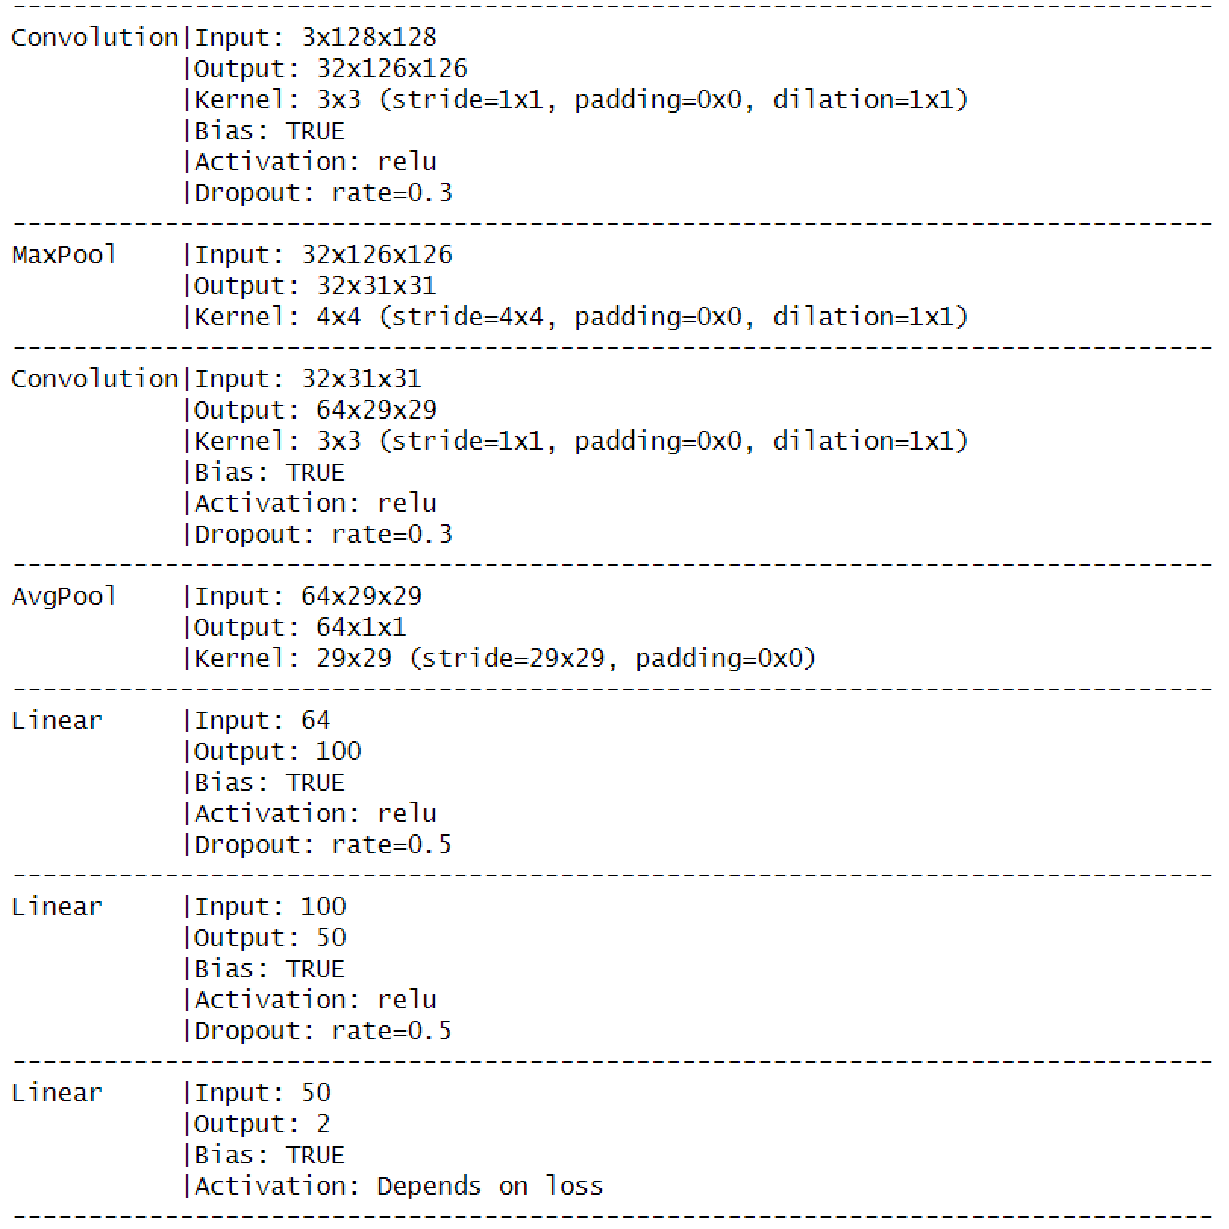
\includegraphics[width=\textwidth]{print.pdf}
	\end{subfigure}
	\hfill
	\begin{subfigure}{0.47\textwidth}
		\centering
		\vspace*{0.2cm}
		\newsavebox{\plotbox} % Create a savebox to store the listing
		\begin{lrbox}{\plotbox}
			\begin{lstlisting}[basicstyle=\footnotesize]
plot(arch, c(3,128,128), 2)
			\end{lstlisting}
		\end{lrbox}
		\fbox{\usebox{\plotbox}}
		\newline
		\vspace*{0.04cm}
		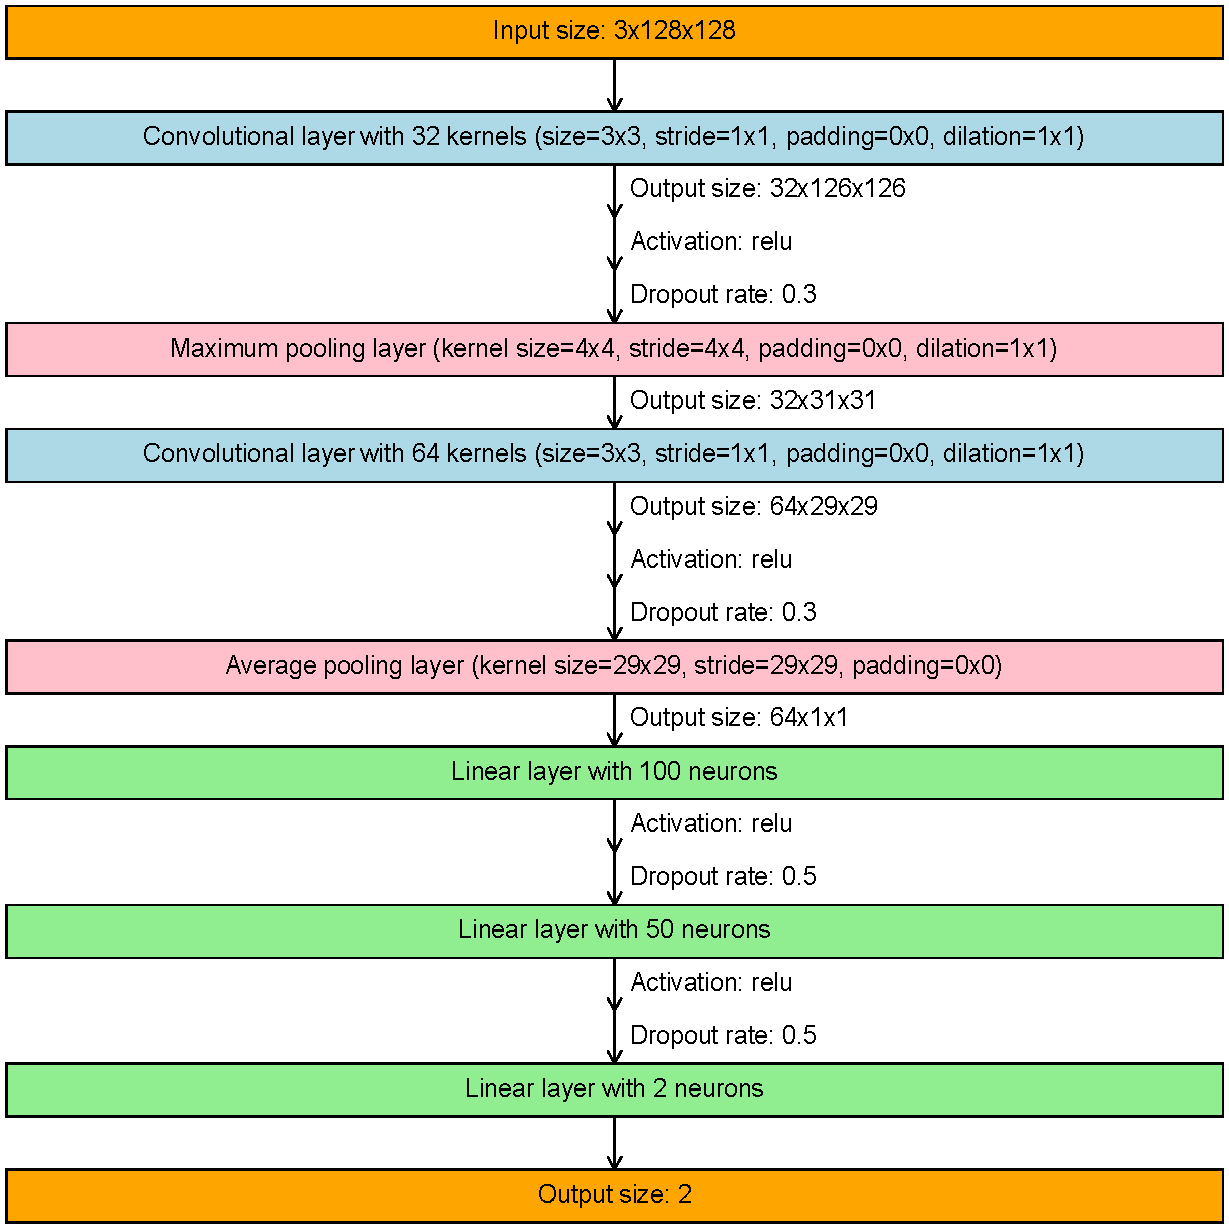
\includegraphics[width=\textwidth]{plot.pdf}
	\end{subfigure}
	\caption{Output of the \fn{print} (left) and \fn{plot} (right) functions for the created CNN architecture and the specified input and output dimensions. The \fn{print} and \fn{plot} functions also work on the S3 object returned by the \fn{cnn} function. In this case, the input and output dimensions don't have to be specified. Instead, the dimensions are derived from the data used for training.}
	\label{printplot}
\end{figure}
This function generates an object that contains the configuration of the entire CNN architecture. This object is then passed to the \fn{cnn} function, which builds and trains the CNN. To create this object, the \fn{create\_architecture} function sequentially combines provided layer objects, which are created using the provided layer functions \fn{conv}, \fn{avgPool}, \fn{maxPool} and \fn{linear}. Each of these layer functions has several arguments (see Table \ref{layers}) that specify the architecture of the layer, but can also be used without specifying any of them. In this case, the unspecified arguments are filled with the default values set within the \fn{create\_architecture} function. For example, a linear layer created with \fn[n\_neurons=128]{linear} will have its unspecified arguments bias, activation, normalization and dropout set to TRUE, "relu", FALSE and 0.0, respectively. These defaults can be overridden in the \fn{create\_architecture} function, which is useful to avoid having to specify the same value in each layer individually. For example, if you want to apply a dropout rate of 0.5 to all linear layers that don't specify the dropout rate themselves, you can set default\_dropout = \fn[linear=0.5]{list}. Note that this only changes the default value for linear layers, leaving the default dropout rate for convolutional layers at 0.0. If you don't want this, you can either also set a different default for convolutional layers (e.g. default\_dropout = \fn[linear=0.5, conv=0.3]{list}) or set the default dropout rate for both linear and convolutional layers to the same value with default\_dropout = 0.5. Note also that although the dropout rate is theoretically a training hyperparameter, I included it in the architecture specification to make it easier to specify individual values for the layers if necessary.

The kernel\_size, stride, dilation and padding arguments of the convolutional and pooling layers can be specified individually for each input dimension. For example, in the case of 2D convolutions, kernel\_size can be set to c(3,5) to generate 3x5 kernels. Alternatively, if only a single value is given, symmetric kernels will be generated. For example, setting kernel\_size to 5 will generate 5x5 or 5x5x5 kernels if the input data provided to the \fn{cnn} function is two or three dimensional. Setting the stride of pooling layers to NULL (also the default value) sets the stride equal to the kernel\_size, which is commonly done for pooling layers.

For the defaults of the other arguments, I have also chosen values that are commonly used and make sense as defaults. For example, there are several things to consider when choosing the default kernel size: First, the kernel size should be greater than 1 so that the layer increases the receptive field of the CNN. This makes sense for a default value, but doesn't mean that a kernel size of 1 should never be used. For example, many well-known architectures use kernels of size 1 for dimension reduction instead of pooling layers. The default kernel size should also be odd, so that it is possible to add symmetrical padding to make the output feature maps have the same size as the input feature maps. Finally, it has been shown that stacking multiple smaller convolutions achieves the same receptive field as a larger convolution, while being computationally cheaper (especially for 2D and 3D convolutions) and introducing more non-linearities, which help the network to model complex functions \citep{simonyanVeryDeepConvolutional2015}. For example, two 3x3 convolutions achieve the same receptive field as a 5x5 convolution, but need only 18 parameters instead of 25. Therefore, 3 - as the smallest, odd number greater than 1 - is a suitable default value for kernel\_size. This can also be seen in architectures such as VGGNet \citep{simonyanVeryDeepConvolutional2015} and ResNet \citep{heDeepResidualLearning2015}, which consist almost entirely of 3x3 convolutions.

To help the user understand the architecture created by the \fn{create\_architecture} function, I implemented \fn{print} and \fn{plot} functions for the resulting R object. These visualize the configuration of each layer in detail, including how the dimensions of an input of specified size changes after each layer (Figure \ref{printplot}). This implementation of the \fn{create\_architecture} and layer functions allows CNN architectures to be specified with minimal code, while still providing a high degree of flexibility and customization.

\section*{Training CNNs}
\addcontentsline{toc}{section}{Training CNNs}

\begin{table}[t]
	\caption{Arguments of the \fn{cnn} function that control the learning process of the network. The defaults are set to reasonable values, but hyperparameters (e.g. learning rate, batchsize, lambda and alpha) usually need to be tuned to avoid convergence problems and improve performance.}
	\centering
	%\renewcommand{\arraystretch}{1.1}
	\resizebox{\textwidth}{!}{
		\begin{tabular}{|lll|}
			\hline
			\textbf{Argument} & \textbf{Explanation}                                                                               & \textbf{Default} \\
			\hline
			%			loss               & Loss function                                                                             & 'mse'   \\
			optimizer          & Optimizer                                                                                 & 'sgd'   \\
			lr                 & Learning rate                                                                             & 0.01    \\
			lr\_scheduler      & Learning rate scheduler                                                                   & NULL    \\
			epochs             & Number of training epochs                                                                 & 100     \\
			early\_stopping    & Stop training early, if loss doesn't improve over specified number of epochs & Inf    \\
			burnin             & Stop training early, if loss isn't below base-loss after specified number of epochs    & Inf     \\
			validation         & Split data into training and validation set to monitor training                           & 0.0     \\
			batchsize          & Number of samples used in each training step                                              & 32      \\
			shuffle            & Shuffle training batches in between epochs                                                & TRUE    \\
			lambda             & Strength of elastic net regularization                                                    & 0       \\
			alpha              & Split of L1 and L2 regularization                                                         & 0.5     \\
			\hline
		\end{tabular}
	}
	
	\label{parameters}
\end{table}

Once the architecture has been specified, the CNN can be built and trained using the \fn{cnn} function I implemented. The arguments of this function include several hyperparameters (Table \ref{parameters}) that influence the training process and the performance of the network. These hyperparameters can be crucial to avoid common problems such as overfitting. For example, early stopping can be used to stop the training process early if the validation loss does not improve over a specified number of epochs, thus saving the network from unnecessary overtraining. This not only saves time but also helps reduce overfitting \citep{prechelt2002early}. Similarly, elastic net regularization, controlled by the lambda and alpha parameters, can help avoid overfitting by reducing the functional complexity of the network \citep{moradi2020survey}. However, improper configuration of the hyperparameters can also lead to reduced model performance and slow down or even prevent convergence during training. While I set the defaults in the \fn{cnn} function to values that should work for many applications (see chapter \pkg{Case Study} for an example), optimal performance typically requires tuning both the CNN architecture and the training hyperparameters. During training, the \fn{cnn} function visualizes both training and validation loss, allowing users to monitor the training process in real time. As an additional reference for comparison, the loss of an intercept-only model is depicted as a baseline. This visualization helps the user to identify potential problems such as lack of convergence or overfitting.

After the training, the \fn{cnn} function returns an S3 object that contains the trained network as well as metadata about the architecture and training process, including the network parameters of the last and the best performing epoch. The S3 object can then be used to make predictions on new data using the \fn{predict} function, or to continue training for additional epochs using the \fn{continue\_training} function. The latter also allows the training data and hyperparameters to be changed for further optimization. Additionally, the \fn{print} and \fn{plot} functions mentioned earlier (Figure \ref{printplot}) are compatible with this object. In this case, the input and output dimensions don't need to be specified and are instead derived from the data used for training.

\section*{Transfer learning}

Training CNNs from scratch often requires large amounts of data, computational resources and time. In many applications, it can be useful to use a network that has already been pre-trained on a large dataset from another task instead. The features that the network has learned from this dataset act as a good starting point and are then fine-tuned during the training on the new dataset, to adapt the network to the task at hand. This approach, called transfer learning, not only minimizes the need for large datasets, but also reduces the time required to train a CNN.

The R package \pkg{torchvision} \citep{falbelTorchvisionModelsDatasets2024} provides several well-known CNN architectures pre-trained on the ImageNet dataset \citep{deng2009imagenet}, such as ResNet \citep{heDeepResidualLearning2015} and MobileNet V2 \citep{sandlerMobileNetV2InvertedResiduals2019}. I made these CNN architectures available in \pkg{cito} by implementing a function called \fn{transfer} that can be used within the \fn{create\_architecture} function similar to the layer functions. In the \fn{transfer} function the user can specify which pre-trained architecture should be used and whether the pre-trained parameters should be frozen. In this case, only the parameters of the linear layers at the end of the network are adjusted during training. It is also possible to initialize these architectures with random parameters instead.

Since the ImageNet dataset consists of RGB images, all pre-trained architectures of the \pkg{torchvision} package require 3-channel inputs such as RGB images. This is a problem because many applications work with data that doesn't fulfill this requirement. To solve this problem, I replace the first convolutional layer of the pre-trained architectures if the data provided to the \fn{cnn} function has a different number of channels. Instead of randomly initializing the weights of the new convolutional layer, I use the channel-wise averages of the pre-trained weights of the replaced layer. This way, as little power as possible is lost from the pre-training. Additionally, I implemented the option to do this even if the data has 3 channels, which is useful for 3-channel data that aren't RGB images, if you want all channels to be treated equally.

\section*{Multimodal neural networks}
\addcontentsline{toc}{section}{Multimodal neural networks}

\begin{figure}
	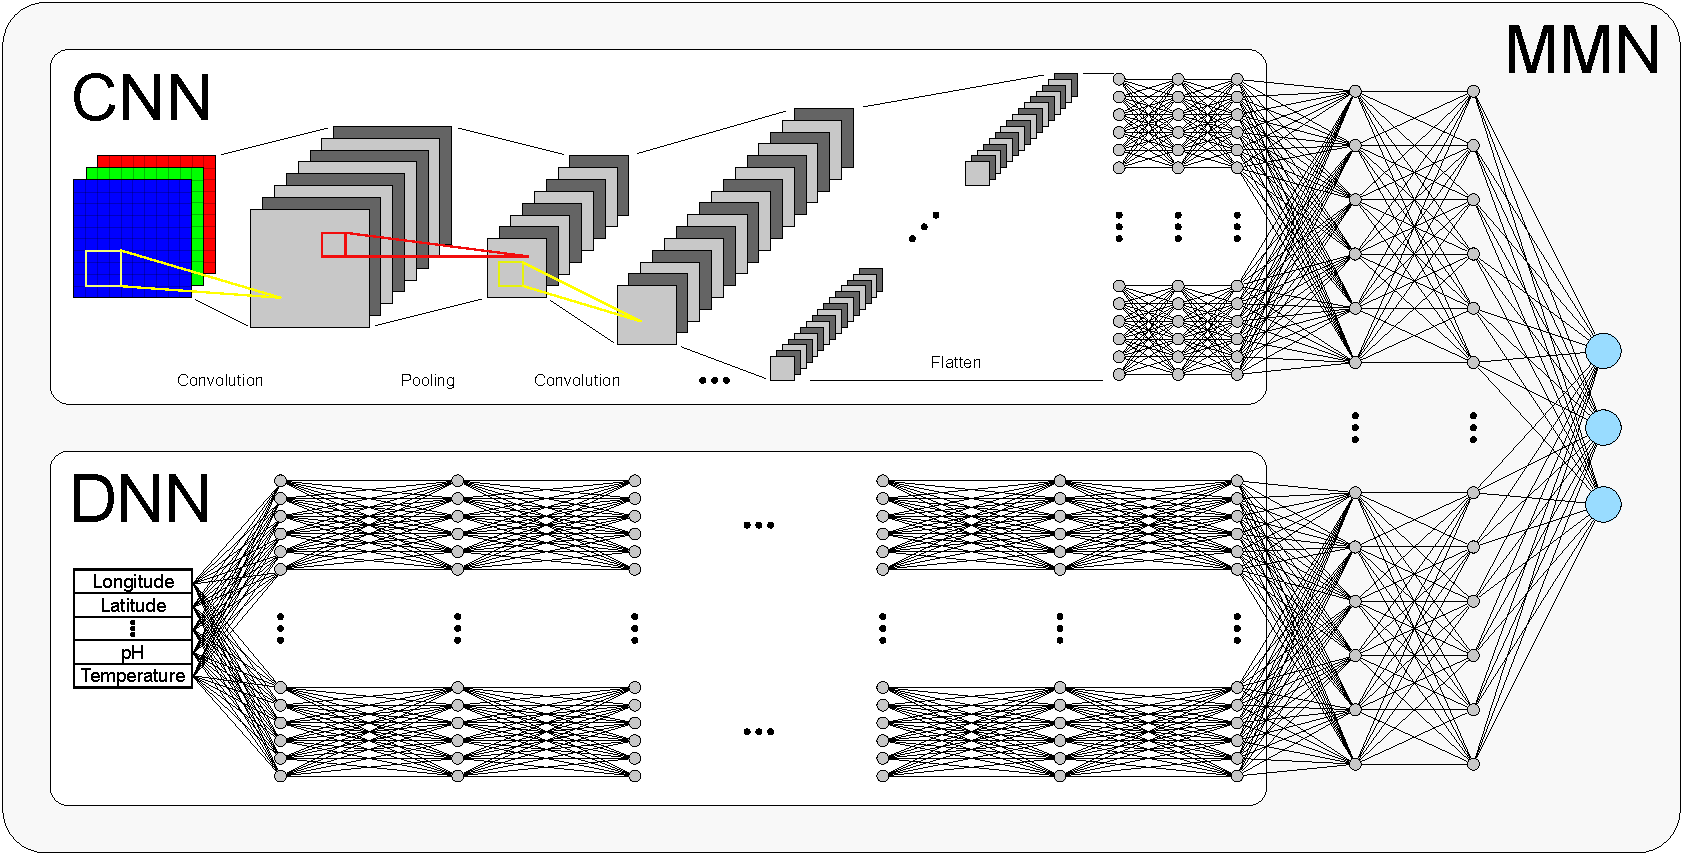
\includegraphics[width=\textwidth]{MMN.pdf}
	\caption{Example of a multimodal neural network that combines a CNN and a DNN to process RGB images and tabular data in the same network. A network like this can be created by $mmn(Y \sim cnn(...) + dnn(...), ...)$. The \fn{mmn} function can combine any number of CNNs and DNNs.}
	\label{MMN}
\end{figure}

An interesting extension of CNNs are multimodal neural networks (MMNs). MMNs combine different neural network architectures to enable the simultaneous processing of data in different formats (e.g. image, tabular, sound). To do this, an appropriate architecture is built for each input format (e.g. CNN for image data, DNN for tabular data). The outputs of the final feature extraction layers of each architecture are then concatenated and serve as input to a linear classifier that makes the final predictions (Figure \ref{MMN}). This allows the network to be trained on all data simultaneously, and to learn interactions between features of different data types. MMNs 

To build and train MMNs in \pkg{cito}, I implemented the \fn{mmn} function. The created MMNs can consist of any number of CNNs and DNNs, which can be specified by the user with a formula. For example, to create an MMN that consists of one CNN and one DNN:

\begin{lstlisting}[literate={~}{{$\sim$}}1]
	mmn(Y ~ cnn(...) + dnn(...), ...)
\end{lstlisting}

where Y is the response variable. Within the \fn{cnn} and \fn{dnn} parts of the formula, the input data and the architecture of the corresponding subnetwork can be specified. The architecture of the linear classifier that combines the subnetworks can be specified in the \fn{mmn} function in the same way as in the \fn{dnn} function (hidden, activation, bias, dropout). The \fn{mmn} function supports the same training hyperparameters as the \fn{dnn} and \fn{cnn} functions (Table \ref{parameters}).

\section*{Package validation}
\addcontentsline{toc}{section}{Package validation}
To test the implementation of CNNs and MMNs, I designed unit tests using the R package \pkg{testthat} \citep{wickhamTestthatGetStarted2011}. The first tests check whether building and training these architectures work for all possible combinations of input data, loss function and training device. To do this, I generate six randomly distributed input data sets to simulate the cases of 1D (e.g. spectrograms), 2D (e.g. images) and 3D (e.g. time series of satellite images) convolutions with 1 or 3 channels each. For each available loss function, I then generate response variables in any acceptable format. For example, the response variable for a binomial loss can be a factor or a matrix filled with either boolean values or ones and zeros. In the tests, one (or more, if the loss function allows different response formats) CNNs are then trained on each available device (CPU, GPU) for each combination of input data and loss function. The CNN architecture used for this is rather simple to reduce computational cost, but includes all available layer types presented above. For each trained CNN, the implemented support functions \fn{print}, \fn{plot}, \fn{predict} and \fn{continue\_training} are also tested to ensure that they run without errors.

Unlike the first tests, which use only randomly generated data to prove that the code is working correctly, the next test uses non-random data to ensure that the networks are able to learn and predict properly. To do this, I generate grey-scale images of either rectangles or ellipsoids. 90\% of the generated images are used to train a CNN, which is then used to predict the class labels of the remaining 10\%. The test is considered successful if the accuracy achieved is greater than 95\%. To train the CNN in this test, I also use some of the supported training techniques, such as elastic net regularization and early stopping.

The final tests ensure that transfer learning is working properly. First, I test whether all the supported architectures of the \pkg{torchvision} package can be loaded and used to build and train a CNN without errors. Afterwards, I conduct an accuracy test similar to the one described above.

The tests for the MMN architecture are mostly the same. The main difference is that instead of a CNN, an MMN consisting of one CNN and one DNN is trained.

\section*{Package availability}
\addcontentsline{toc}{section}{Package availability}
The current version of \pkg{cito} (1.1) can be downloaded from the comprehensive R archive network (CRAN). My implementation of CNNs and MMNs are added in version 1.1.1, which can be found on GitHub (\url{https://github.com/citoverse/cito}) and are planned to be included in the next CRAN release.

\chapter*{Case study}
\addcontentsline{toc}{chapter}{Case study}
\newsavebox{\cnn} % Create a savebox to store the listing
\begin{lrbox}{\cnn}
	\begin{lstlisting}[literate={~}{{$\sim$}}1]
mobilenet <- create_architecture(transfer("mobilenet_v2", freeze = FALSE))

cnn(X = spectra,
    Y = tabular_data[["species"]],
    architecture = mobilenet,
    loss = "softmax",
    validation = 0.1,
    early_stopping = 3,
    device = "cuda",
    batchsize = 16) -> cnn.fit
		
mmn(formula = tabular_data[["species"]] ~ 
              cnn(X = spectra, architecture = mobilenet) +
              dnn(formula = ~ longitude + latitude, data = tabular_data),
    loss = "softmax",
    validation = 0.1,
    early_stopping = 3,
    device = "cuda",
    batchsize = 8) -> mmn.fit
	\end{lstlisting}
\end{lrbox}

\newsavebox{\dnn} % Create a savebox to store the listing
\begin{lrbox}{\dnn}
	\begin{minipage}{\wd\cnn}
		\begin{lstlisting}[literate={~}{{$\sim$}}1]
dnn(formula = species ~ longitude + latitude,                             
    data = tabular_data,
    loss = "softmax",
    validation = 0.1,
    early_stopping = 3,
    device = "cuda",
    batchsize = 16) -> dnn.fit
		\end{lstlisting}
	\end{minipage}
\end{lrbox}

\noindent After discussing the implementation of CNNs and MMNs in \pkg{cito}, I now want to demonstrate the workflow of using \pkg{cito} for an ecological application that requires these architectures. The example I have chosen is the classification of bird species based on audio recordings. When processing audio recordings, models are often trained on extracted features rather than raw audio signals. A common approach is to transform the audio signals into 2D frequency-time spectrograms, which are spatially structured in the frequency and time dimensions, making them a good application for CNNs.

\section*{Data}
\addcontentsline{toc}{section}{Data}
The data I used for this case study came from the BirdCLEF 2024 Kaggle competition \citep{birdclef-2024}. This dataset consists of over 20,000 audio recordings of bird calls from the \url{xeno-canto.org} website. From each recording, I sampled a random 10 second chunk and transformed them into Mel spectrograms using the R package "torchaudio" \citep{keydanaTorchaudioInterfacePytorchs2023}. Mel spectrograms are frequency-time spectrograms in which the frequency values are transformed to the Mel scale, which more accurately represents how humans perceive sound, as humans can detect frequency differences better at lower frequencies \citep{stevensScaleMeasurementPsychological1937}. I took the hyperparameters used for this transformation (e.g. n\_fft, n\_mels) from the winning solution of the Kaggle competition. After the transformation, I min-max normalized each spectrum to have values between 0 and 1. In addition to the audio recordings, the dataset also provides a quality rating of the recordings and the coordinates of the location where they were recorded. After discarding audio recordings with bad ratings or missing longitude/latitude values, I ended up with 21166 samples for 177 different bird species.

\section*{Models}
\addcontentsline{toc}{section}{Models}
I used this data to train the three model architectures that \pkg{cito} now supports: Fully connected neural networks were trained on the coordinates, convolutional neural networks were trained on the Mel spectrograms, and multimodal neural networks were trained on both the coordinates and the Mel spectrograms. In this case study, I primarily used the default values of the hyperparameters to simulate the case of an inexperienced user who wants to train deep neural networks in a single line of code without spending a lot of time tuning the hyperparameters:

\begin{figure}[p]
	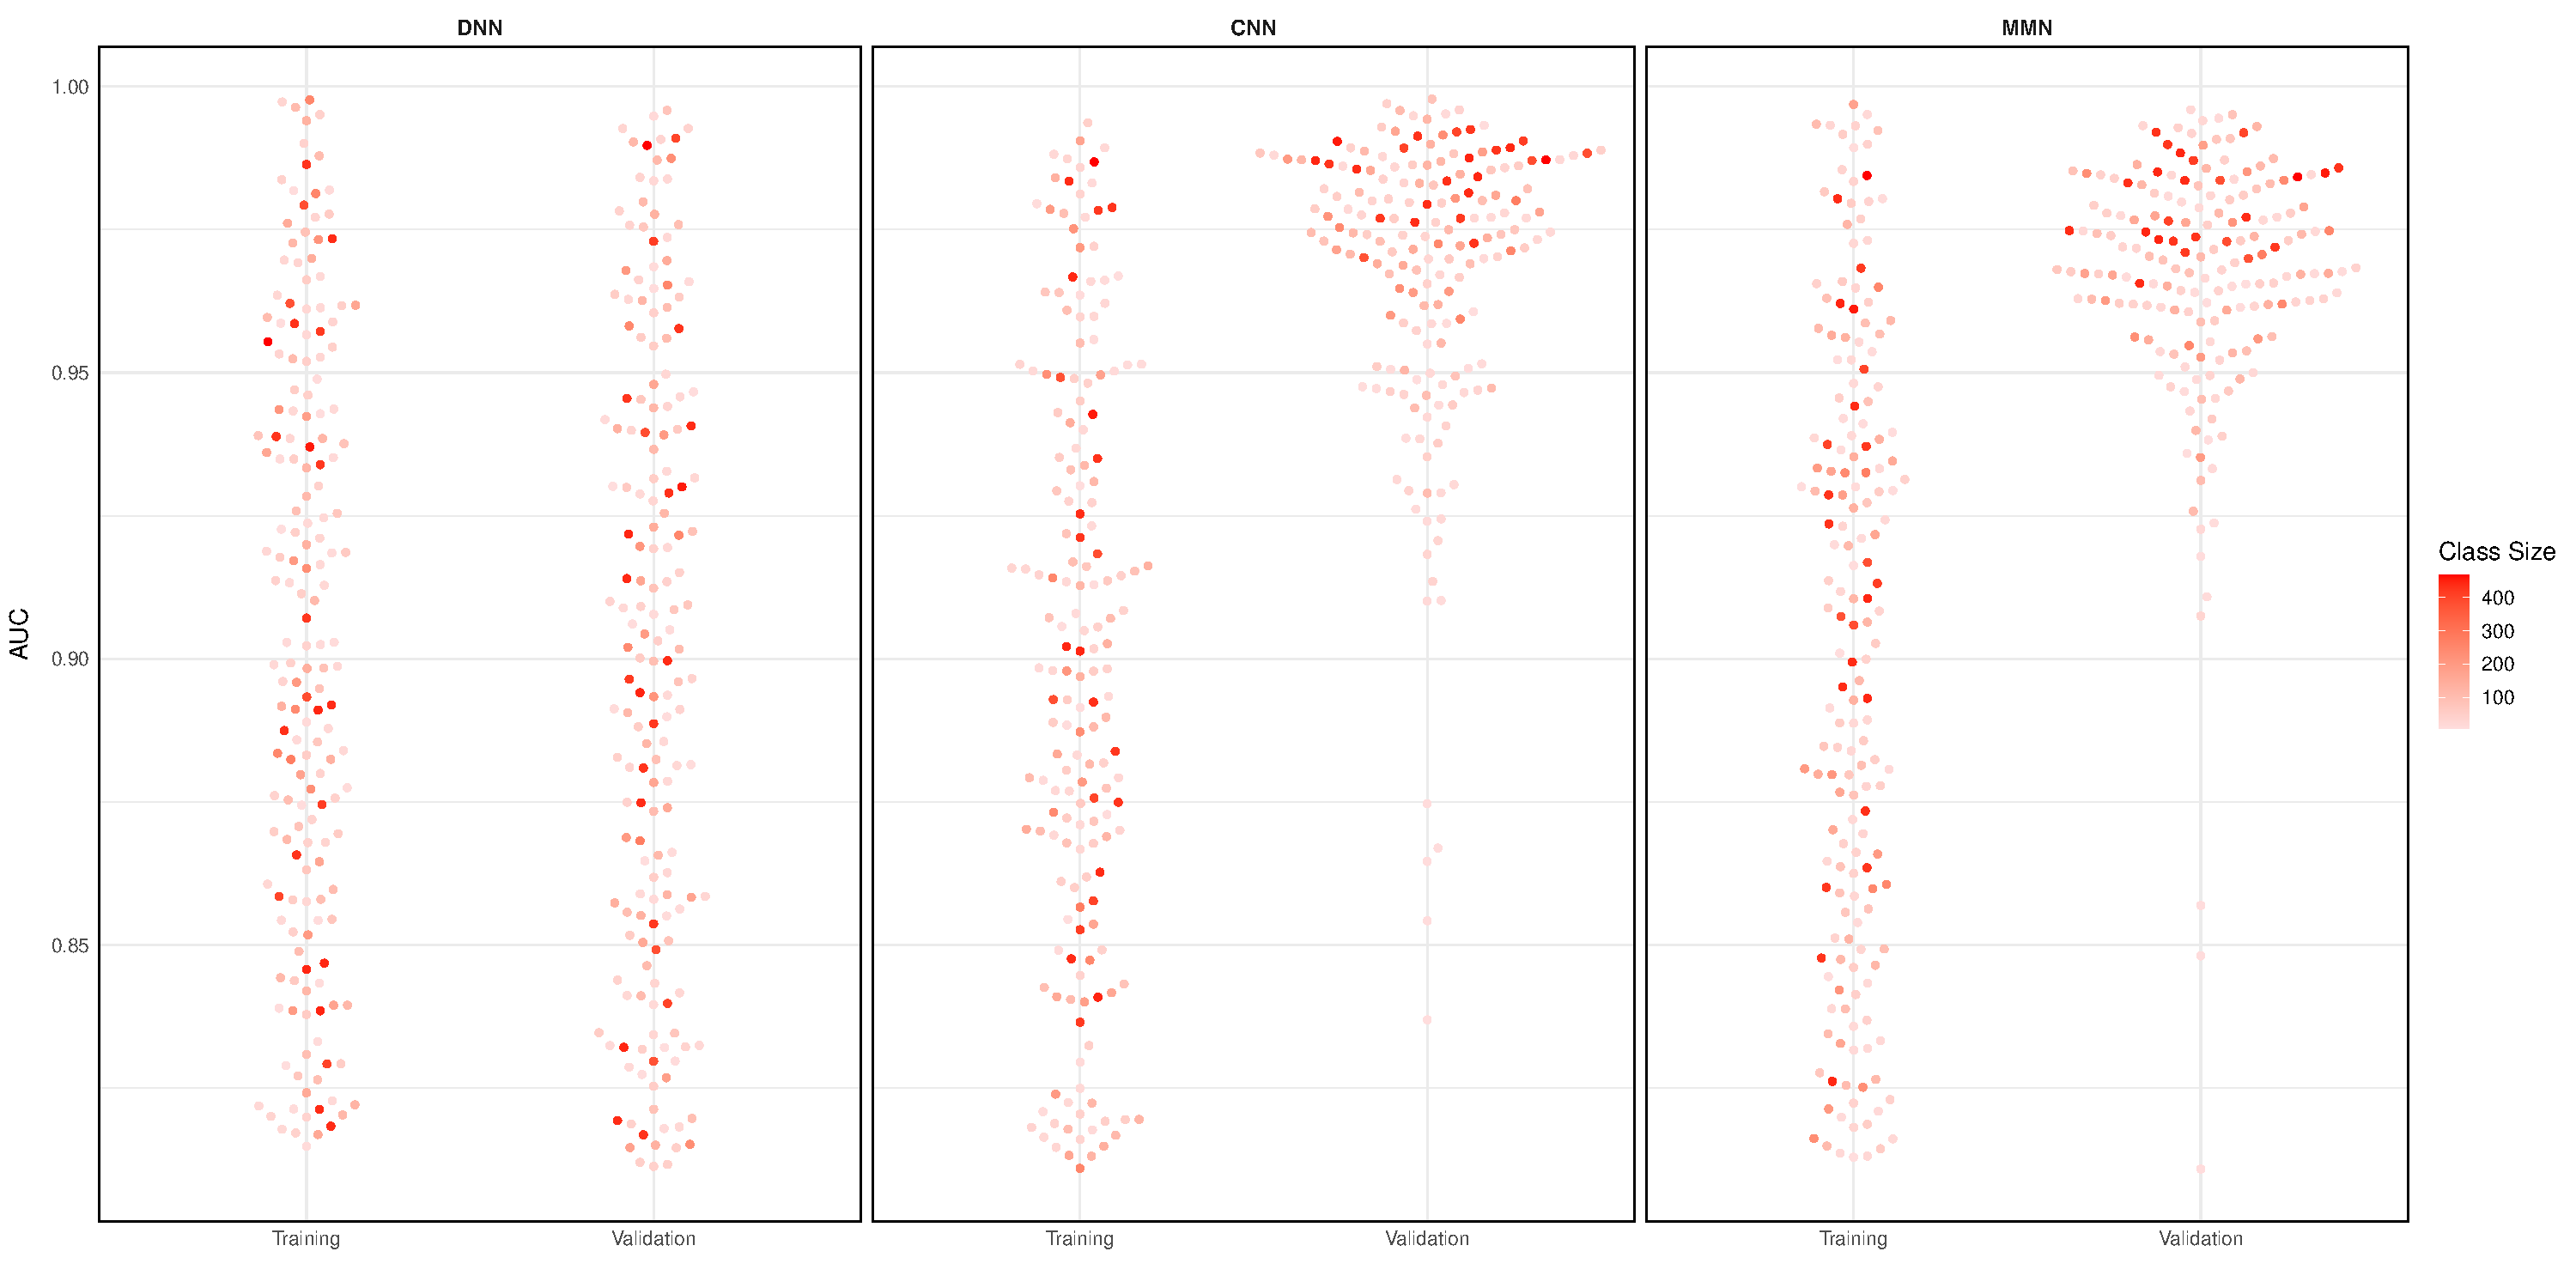
\includegraphics[width=\textwidth]{../analysis/results/figures/auc_beehive.pdf}
	\caption{Performance comparison of the three architectures implemented in \pkg{cito} (DNN, CNN, MMN) for bird species classification. DNNs were trained on the coordinates of the location of the audio recordings, CNNs were trained on the Mel spectrograms of the audio recordings, and MMNs were trained on both. Each architecture was trained 5 times in a 5-fold stratified cross-validation. For each of the 5 trained models, predictions were made for the 4 training folds, and the omitted validation fold. The predictions of the 5 models were combined to calculate two one-vs-all AUC values for each of the 177 bird species; one for the training and one for the validation predictions. These AUC values are shown, color coded according to the number of samples in the dataset belonging to the species.}
	\label{beehive}
	\rule{\textwidth}{1pt} 
	\newline
	\resizebox{\textwidth}{!}{\usebox{\dnn}}
	\resizebox{\textwidth}{!}{\usebox{\cnn}}
\end{figure}

\newpage

%\begin{figure}[h]
%	\centering
%	\resizebox{\textwidth}{!}{\usebox{\dnn}}
%\end{figure}

%\begin{figure}[h]
%	\centering
%	\resizebox{\textwidth}{!}{\usebox{\cnn}}
%\end{figure}

\begin{figure}[ht]
	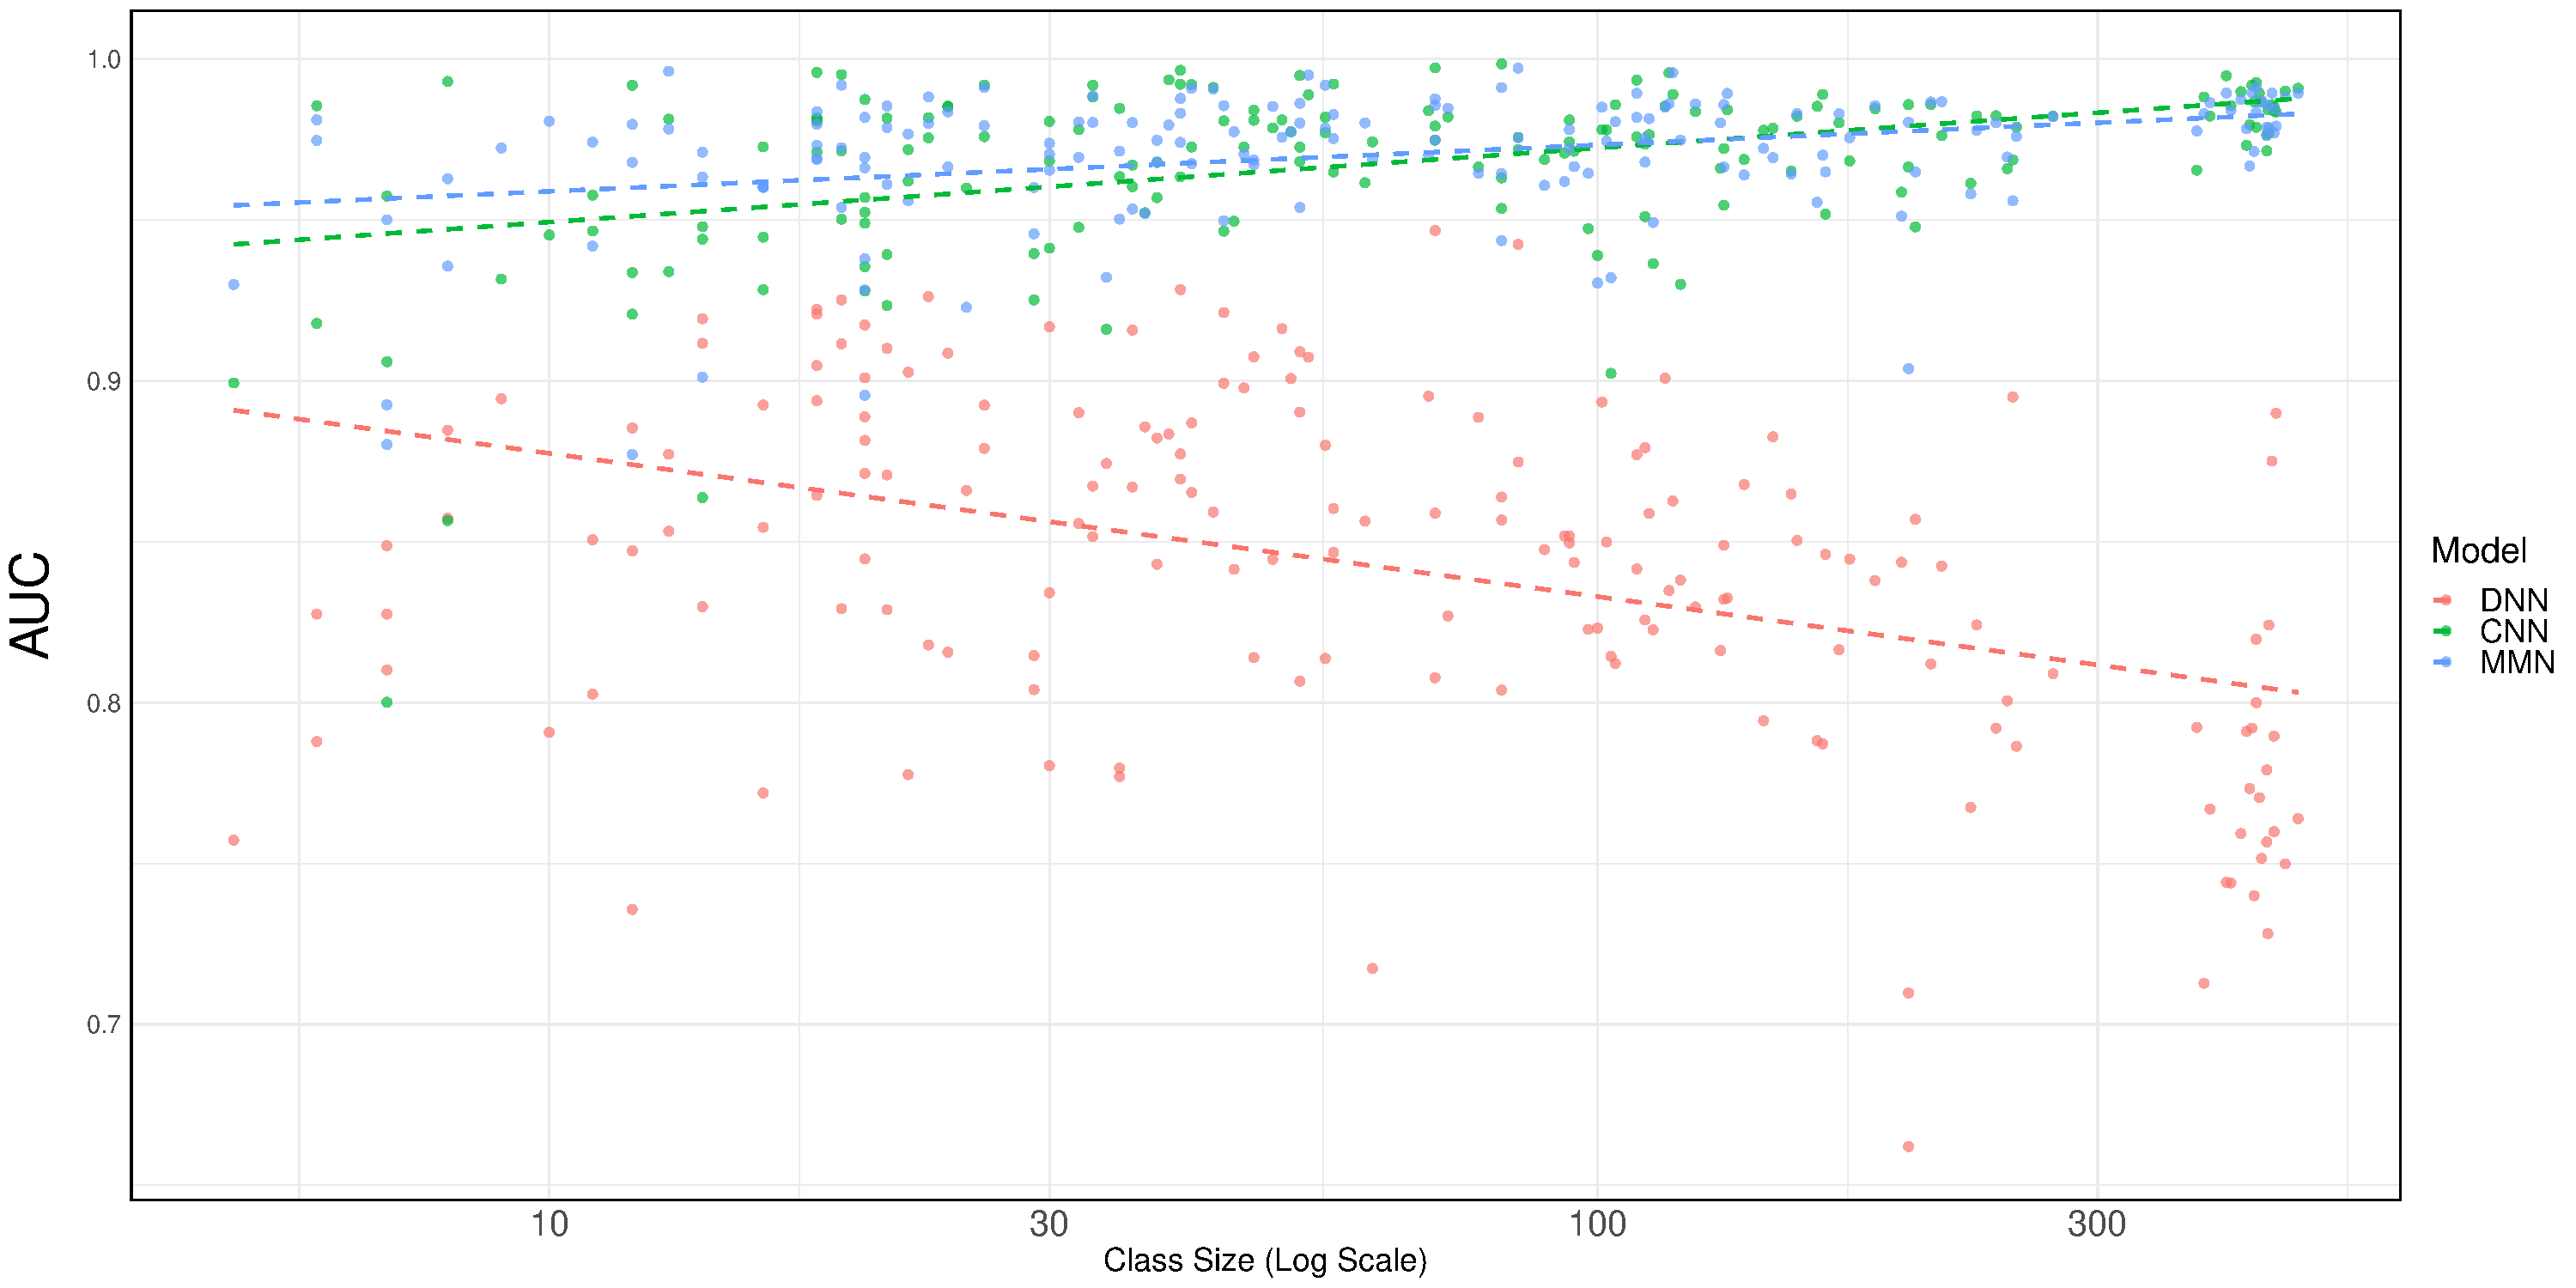
\includegraphics[width=\textwidth]{../analysis/results/figures/auc_classSize.pdf}
	\caption{Relationship between class size and AUC values of the 177 bird species. Only the AUC values calculated for the predictions of the validation folds of the cross-validation are shown. The dotted lines illustrate the linear effect $AUC \sim class\,size$ for the three architectures.}
	\label{classSize}
\end{figure}

To demonstrate the transfer learning option, I used the MobileNet V2 \citep{sandlerMobileNetV2InvertedResiduals2019} architecture with pre-trained weights for the CNNs (and the CNN part of the MMNs). For DNNs (and the DNN part of the MMNs) I used the default architecture (two hidden layers with 50 neurons each). I set device = "cuda" to enable training on GPUs and changed the batchsize to 16 (8 for MMNs), as the GPUs I used did not have enough memory to support the default batchsize of 32. I also set validation=0.1 and early\_stopping=3. This caused the models to use 10\% of the provided training data as a validation set and to stop training early if the loss on that validation set has not improved over the last 3 epochs, which not only reduces the training time of these models but also helps to reduce overfitting.

\section*{Evaluation}
\addcontentsline{toc}{section}{Evaluation}
I evaluated the network architectures using 5-fold cross-validation on the dataset. As the dataset is highly unbalanced, with class sizes ranging from 5 to 466, I used stratified sampling to ensure that class distributions were preserved in each fold and that each fold contained at least one sample of each bird species. In the cross-validation, I trained 5 models for each architecture. Each model was used to make predictions on the 4 folds used for its training, as well as on the omitted validation fold. I then computed one-vs-all AUC (area under the receiver operating characteristic curve) values for each of the 177 bird species on the combined training and validation predictions, respectively. The averages of these AUC values were used to evaluate the training and validation performance of each architecture. In the Kaggle competition, the macro-average AUC was also used as metric to evaluate model performance.

\section*{Results}
\addcontentsline{toc}{section}{Results}

I made three observations when comparing the performance of the architectures: 1) On the validation folds, the MMN performs slightly better than the CNN and both perform much better than the DNN (Figure \ref{beehive}). The macro-average AUC values on the validation folds for the MMN, CNN and DNN are 0.970, 0.968 and 0.842, respectively. 2) While all architectures perform worse on the validation folds, the difference in macro-average AUC between the training and validation folds is largest for the CNN, slightly smaller for the MMN and much smaller for the DNN (Figure \ref{beehive}). The differences in macro-average AUC for the CNN, MMN and DNN are -0.029, -0.022 and -0.009, respectively. 3) For all three architectures, the size of a class has a significant linear effect on the corresponding validation AUC. However, while this effect is positive for the CNN and MMN, it is negative for the DNN (Figure \ref{classSize}). The computed linear effects for the CNN, MMN and DNN are $6.350\times10^{-5}$, $4.298\times10^{-5}$ and $-2.134\times10^{-4}$, respectively.

\section*{Code availability}
\addcontentsline{toc}{section}{Code availability}
The code I used to preprocess the data, train the networks and generate the results can be found in the Appendix or on GitHub: \url{https://github.com/ArminSchenk/BirdSongRecognition}

\chapter*{Discussion and conclusion}
\addcontentsline{toc}{chapter}{Discussion and conclusion}
In this work, I presented the implementation of CNN and MMN architectures in the R package \pkg{cito}. Building and training CNNs previously required users to have extensive knowledge of complex deep learning frameworks such as PyTorch or TensorFlow. With the simple interface I provide, this is no longer necessary. Because of the \pkg{torch} backend and the GPU support it provides, \pkg{cito} can train these large networks as efficiently as the complex frameworks. I also provide the ability to use transfer learning by integrating several pre-trained models. To address the current trend towards MMNs, I have implemented a function that can combine several DNN and CNN architectures into a MMN. Using bird species classification as an example, I demonstrated how little code is required when using \pkg{cito} to train good performing CNN-based classifiers.

In my case study the MMN and CNN architectures performed much better than the DNN architecture. This was expected since the DNNs were only trained on the coordinates, which obviously aren't enough for a complex task such as species classification, because several different bird species can occur at the same location. This is probably also the reason why the DNN performed worse for the more common bird species. Since common bird species are usually also wider spread, the classification based on coordinates alone becomes more difficult. However, I also showed that the MMN architecture performed slightly better than the CNN on the validation folds and slightly worse on the training folds. While the CNN was trained using only the Mel spectrograms of the audio recordings, the MMN was trained using both the Mel spectrograms and the coordinates of the recording location. The slightly better validation performance and slightly worse training performance could indicate that the MMN was able to use the coordinate values to reduce overfitting. A possible explanation could be that the coordinates help the MMN to better identify local bird call dialects. Recently, \citet{sastryBirdSATCrossViewContrastive2024} proposed a framework for bird species classification and ecological mapping that also uses a multimodal approach including metadata (coordinates and time) in addition to ground-level bird images and satellite images, supporting my findings that including metadata (such as coordinates) can be useful for bird species classification. Apart from including metadata, multimodal architectures have also been used to combine audio and visual data for bird species classification \citep[e.g.,][]{bold2019cross}cand have also found success in other ecological applications such as species distribution modeling \citep[e.g.,][]{zhangNovelMultimodalSpecies2022}. Since MMNs are still relatively new, more work  still has to be done to better understand for what applications and under what conditions MMNs can and should be used. Implementing MMNs in \pkg{cito} makes them more accessible, which contributes to this progress.

In my case study, the MNN achieved a high macro-average AUC of 0.970 on the validation folds of the 5-fold cross-validation. However, these results should not be compared to the results of the BirdCLEF2024 Kaggle competition (macro-average AUC of winning team: 0.690), as the models of the competition were evaluated on a separate test set, which has significant differences from the training set I performed my evaluation via cross-validation on: 1) The test set contains only the audio files, not the coordinates. This makes it impossible to evaluate the DNNs and MMNs I trained on the test set, as they need these to make predictions. 2) Unlike the training set, which contains sound recordings from all over the world, the test set only contains sound recordings from the Western Ghats of India. This local blocking of the test set could reduce model performance, as a model trained on the global data could overfit to global patterns, such as background noise or local dialects of bird calls, that are not present in the local region of the test set. 3) The sound recordings in the test set have a fixed length of 4 minutes, whereas the median length of the sound recordings in the training set is only 22.7 seconds. A large proportion of the training recordings are shorter or only slightly longer than 10 seconds, so it can be expected that the randomly sampled 10-second chunk will contain at least parts of the bird call that can be used for prediction. The probability that a random 10-second chunk of the 4-minute audio recordings in the test set will contain parts of the bird call, rather than just noise, is lower. The winning team in the Kaggle competition dealt with this problem by dividing the audio recordings into 10-second chunks and then averaging the predictions of these chunks. However, as there may be chunks with little or no parts of the bird call and mostly background noise, this can increase the uncertainty of the final predictions and reduce the overall performance measured by AUC. 

While there are several other R packages that provide an interface as user-friendly as \pkg{cito}s for DNNs, there is not yet a single other R package that does so for CNNs. The \pkg{mlr3torch} \citep{fischerMlr3torchDeepLearning2024} package comes closest. While it provides an easy way to use custom DNNs and the pre-trained CNNs from the \pkg{torchvision} package in a \pkg{mlr3} \citep{mlr3} workflow, using custom CNNs is as complex as using the large deep learning frameworks. Furthermore, the pre-trained CNNs are restricted to 3-channel, 2D input (RGB images) and can only be used for classification, whereas \pkg{cito} allows the pre-trained models to be used for any number of input channels (although still restricted to 2D input) and also for regression. The \pkg{mlr3} framework (including \pkg{mlr3torch}) focuses on creating pipelines to streamline the entire machine learning workflow, built modularly with independent components ranging from data preprocessing to hyperparameter tuning to performance evaluation and visualization. The chosen learner, such as a neural network, is just one of these independent components. While this flexible design can be useful for machine learning tasks, it adds another layer of complexity that \pkg{cito} tries to avoid.  As such, the \pkg{mlr3} framework is aimed at machine learning engineers and data scientists, whereas \pkg{cito} is aimed at practical researchers, such as ecologists, who often don't have extensive machine learning experience and therefore need a simple interface like \pkg{cito}s to make complex architectures such as CNNs and MMNs accessible. In the future, more neural network architectures are planned to be implemented in \pkg{cito}, which will also allow the \fn{mmn} function to combine even more types of data (e.g. recurrent neural networks for time-series data). 

Now I want to talk about some limitations of \pkg{cito}. As I mentioned, transfer learning is currently only available for 2D input data. Although this already covers many applications, there has been work highlighting the use of transfer learning for 1D \citep[e.g., ][]{fawazTransferLearningTime2018, weimannTransferLearningECG2021a} and 3D \citep[e.g., ][]{kopukluResourceEfficient3D2021a, haraCanSpatiotemporal3D2018} CNNs. Therefore, pre-trained 1D and 3D CNN architectures should be integrated in \pkg{cito} in the future. This has not been done yet, because there are no R packages that provide 1D or 3D pre-trained models implemented with the \pkg{torch} backend, similar to \pkg{torchvision} for 2D models. There are, however, pre-trained models available in python (e.g., \url{https://github.com/okankop/Efficient-3DCNNs}). These could be integrated in \pkg{cito}, but this would require manually rebuilding the architectures with \pkg{torch} and then importing the pre-trained parameters.

Another limitation of \pkg{cito} is the lack of integrated xAI methods for CNNs that help to explain the behavior of a model. For example, xAI methods can be used to detect whether the model is basing its predictions on relevant features rather than overfitting to noise or irrelevant features \citep[e.g., basing the classification of images of wolves or dogs on whether or not there is snow in the background ][]{ribeiroWhyShouldTrust2016}. xAI methods can also help to detect whether the model has learned an unintentional bias from the data \citep[e.g., gender bias in the classification of images of doctors or nurses ][]{selvarajuGradCAMVisualExplanations2020}. Being able to detect these problems is crucial to building trust in model predictions, especially for critical applications such as medicine or autonomous driving. Currently, there are no xAI methods for CNNs implemented in \pkg{cito}. However, the R package \pkg{innsight} \citep{koenenInterpretingDeepNeural2024} implements several xAI methods to explain individual predictions, such as Layer-Wise Relevance Propagation \citep{bachPixelWiseExplanationsNonLinear2015a} or SmoothGrad \citep{smilkovSmoothGradRemovingNoise2017}, which can be used for \pkg{cito}s custom CNNs (pre-trained CNNs and MMNs are based on a different \pkg{torch} class, which isn't supported). In the future, it is planned to integrate some of these xAI methods directly into \pkg{cito} to support all model architectures and reduce dependency on other packages.

In many fields, such as medicine, finance and autonomous driving, decisions made based on model predictions can have critical consequences. Therefore, it is important to provide prediction intervals that quantify the uncertainty of model predictions, which is not yet possible in \pkg{cito}. For DNNs, \pkg{cito} can already compute confidence intervals for predictions using bootstrapping. While this method could be extended to CNNs, the high computational cost of training CNNs makes it impractical. Moreover, confidence intervals only account for epistemic (systematic) uncertainty and not aleatoric (statistical) uncertainty. To generate accurate prediction intervals, both sources of uncertainty must be taken into account. Therefore, future plans include the integration of methods for computing prediction intervals, especially those that don't require the training of multiple CNNs, such as Monte Carlo Dropout \citep{galDropoutBayesianApproximation2016} or Conformal Prediction \citep{shafer2008tutorial}.

In conclusion, I extended the \pkg{cito} package to include user-friendly interfaces for building and training CNNs and MMNs. This makes these complex neural network architectures more accessible to researchers without extensive knowledge of deep learning frameworks and hopefully contributes to future research of these models in ecology.

\newpage
\renewcommand{\bibname}{References}
\addcontentsline{toc}{chapter}{References} % Add Bibliography to the table of contents
% this is the style file. If you need to change something, google if the file you need is already there. If not (very uncommon) google makebst.
\bibliographystyle{chicago} 
\bibliography{../literature/literature} % Reference the BibTeX library file

\chapter*{Appendix}
\addcontentsline{toc}{chapter}{Appendix}
\lstdefinestyle{Rstyle}{
	language=R,
	basicstyle=\ttfamily\small,
	commentstyle=\color{green!60!black},
	stringstyle=\color{orange},
	showstringspaces=false,
	breaklines=true,
	frame=single,
	numbers=left,
	numberstyle=\tiny\color{gray},
	literate={/}{/}{1}  % Make "/" regular
			 {_}{\_}{1} % Make "_" regular
}
\lstset{style=Rstyle}
\section*{1-dataPreparation.R}
\lstinputlisting{../analysis/1-dataPreparation.R}
\newpage
\section*{2-buildingDNNs.R}
\lstinputlisting{../analysis/2-buildingDNNs.R}
\newpage
\section*{2-buildingCNNs.R}
\lstinputlisting{../analysis/2-buildingCNNs.R}
\newpage
\section*{2-buildingMMNs.R}
\lstinputlisting{../analysis/2-buildingMMNs.R}
\newpage
\section*{3-visualisation.R}
\lstinputlisting{../analysis/3-visualisation.R}
\newpage
\section*{utils.R}
\lstinputlisting{../analysis/utils.R}
\newpage

\chapter*{Declaration of independence}
\addcontentsline{toc}{chapter}{Declaration of independence}
Ich habe die Arbeit selbstständig verfasst, keine anderen als die angegebenen Quellen und Hilfsmittel benutzt und bisher keiner anderen Prüfungsbehörde vorgelegt. Außerdem bestätige ich hiermit, dass die vorgelegten Druckexemplare und die vorgelegte elektronische Version der Arbeit identisch sind, dass ich über wissenschaftlich korrektes Arbeiten und Zitieren aufgeklärt wurde und dass ich von den in §26 Abs. 5 vorgesehenen Rechtsfolgen Kenntnis habe.

\vspace{2cm}
\begin{flushright}
	\renewcommand{\arraystretch}{1.3}
	\begin{tabular}{ccc}
		\hline
		\hspace*{2cm}&Unterschrift&\hspace*{2cm}\\
	\end{tabular}
\end{flushright}


% Note: all files can be anywhere, just give the full path.


\end{document}
